\documentclass[a4paper]{article}
\usepackage[english]{babel}
\usepackage[table]{xcolor}
% Load the VUB package.
% This has many options, please read the documentation at
% https://gitlab.com/rubdos/texlive-vub
\usepackage{vub}
\usepackage{hyperref}
\usepackage{subcaption}
\usepackage{xcolor} % to access the named colour LightGray
\definecolor{LightGray}{gray}{0.9}
\usepackage{minted}

% Some highly suggested packages, please read their manuals.
\usepackage{cleveref}
\usepackage[natbib,style=apa]{biblatex}
%\addbibresource{bibliography.bib}


\title{Statistics}
\subtitle{Methods for Scientific Research}
\author{Gérard Lichtert}
\date{\today}
\faculty{Sciences and Bio-Engineering Sciences} % Note, no
\begin{document}
\maketitle
\begin{abstract}
Before reading, perhaps it is interesting to know the following: I drew the following question sets:
    \begin{figure}[H]
        \centering
        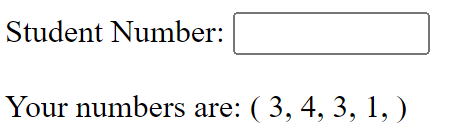
\includegraphics[width=0.3\linewidth]{images/Screenshot 2023-12-02 025750.png}
        \caption{Generated questions}
        \label{fig:qs}
    \end{figure}
Furthermore, I used Python version 3.12 in Jupyter Notebook and the appropriate libraries to answer the questions. I will provide the code that I used to answer the questions so that the answers can be verified, except for some cases where the generated samples could differ from yours. The libraries and the versions used will be added to Appendix A. With regard to the questions, they will always be copied from the assignment, as well as some context.
\end{abstract}
\newpage
\tableofcontents
\newpage
\section{Question 1}
\subsection{General information}
\begin{itemize}
    \item The data file contains the times it takes for participants to respond to two versions of a web form. We will call this 'response time' from now on.
    \item The dataset used for this question is Question1\_3.txt. 
\end{itemize}
\subsection{Make a maximum of two appropriate plots to show how the data are distributed and to show the difference between the two web forms. Explain why you used this type of plot. (2+2pts)}
To start analysing our data, let us import the data to get some general information about our dataset.
\begin{listing}[H]
\begin{minted}[
baselinestretch=1.2,
frame=lines,
framesep=2mm,
bgcolor=LightGray,
fontsize=\footnotesize,
linenos
]
{python}
import pandas as pd
df = pd.read_csv('datasets/Question1_3.txt', sep="\t", header=0)
df.describe()
\end{minted}
\caption{Describing the datasets}
\label{listing:q1describe}
\end{listing}
\begin{table}[H]
    \centering
    \begin{tabular}{|c|c|c|}
        \hline
         & interface1 & interface2\\
         \hline
         count & $20$ & $20$\\
         \hline
         mean & $30.687$ & $44.765$\\
         \hline
         std & $13.112$ & $47.884$\\
         \hline
         min	& $17.89$ & $18.1$\\
         \hline
         $25\%$ & $20$ &	$22.35$\\
         \hline
         $50\%$ & $28.335$ & $31.75$\\
         \hline
         $75\%$ & $36.9$ & $43.2$\\
         \hline
         max & $68.74$ & $234.7$\\
         \hline
    \end{tabular}
    \caption{Data description}
    \label{tab:q1description}
\end{table}
As we can see in Table \ref{tab:q1description}, there are $20$ participants total. The means of the response times are $30.687$ and $44.765$ for the first interface and second interface, respectively. The standard deviation is between $13.11$ and $47.88$. The rest is not discussed, as it will be shown in the plots below.\newline\newline
For the first plot, I will be using a boxplot to show the distribution of data. I used this plot because it shows the median, the $25$- and $75$-quartile, range, and outliers. This gives a good overview of the data. I initially tried a histogram as well, but as the sample is relatively small, it didn't give a good overview of the distribution of data.
\newline
\begin{listing}[H]  
\begin{minted}[
baselinestretch=1.2,
frame=lines,
framesep=2mm,
bgcolor=LightGray,
fontsize=\footnotesize,
linenos
]
{python}
import matplotlib.pyplot as plt
bp = plt.boxplot([df['interface1'], df['interface2']], labels=['1', '2'], showmeans=True,
    meanline=True)
plt.title('Boxplot of the datasets')
plt.legend([bp['means'][0], bp['medians'][0]], ['Mean', 'Median'])
plt.xlabel('interface')
plt.ylabel(xlabel)
plt.show()
\end{minted}
\caption{Plotting a boxplot}
\label{listing:q1boxplot}
\end{listing}
\begin{figure}[H]
    \centering
    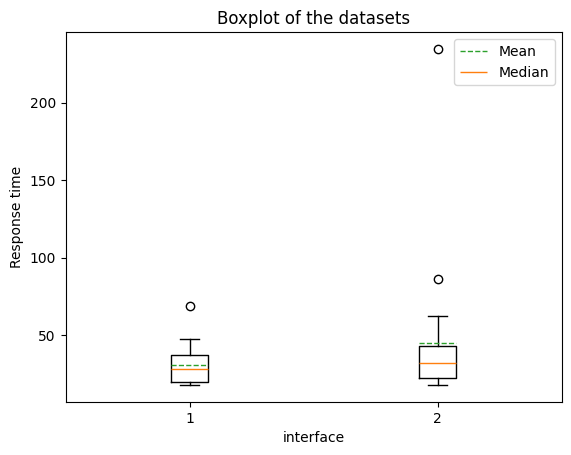
\includegraphics[width=0.8\textwidth]{images/q1boxplot.png}
    \caption{Boxplot of the interfaces}
    \label{fig:q1boxplot}
\end{figure}
In figure \ref{fig:q1boxplot}, we can see that the ranges start around the same response time; however, the end of the range differs. The $25$-quantile and the median are about the same, but the $75$-quantile of the second interface is greater than the $75$-quantile of the first interface. \newline
As for my second plot to show how the data is distributed, I chose 11 plots. I chose this plot to visually see whether the data follows the normal distribution. This is important for other statistical tests I might have to use.
\begin{listing}[H]  
\begin{minted}[
baselinestretch=1.2,
frame=lines,
framesep=2mm,
bgcolor=LightGray,
fontsize=\footnotesize,
linenos
]
{python}
import statsmodels.api as sm
sm.qqplot(df['interface1'], line=('s'))
plt.title('QQ-plot for interface 1')
plt.ylabel('response time')
plt.show()
\end{minted}
\caption{Plotting a the QQ-plot for interface1}
\label{listing:q1QQ1}
\end{listing}
\begin{listing}[H]  
\begin{minted}[
baselinestretch=1.2,
frame=lines,
framesep=2mm,
bgcolor=LightGray,
fontsize=\footnotesize,
linenos
]
{python}
sm.qqplot(df['interface2'], line=('s'))
plt.title('QQ-plot for interface 2')
plt.ylabel('response time')
plt.show()
\end{minted}
\caption{Plotting a the QQ-plot for interface2}
\label{listing:q1QQ2}
\end{listing}
\begin{figure}[H]
    \begin{subfigure}{0.5\textwidth}
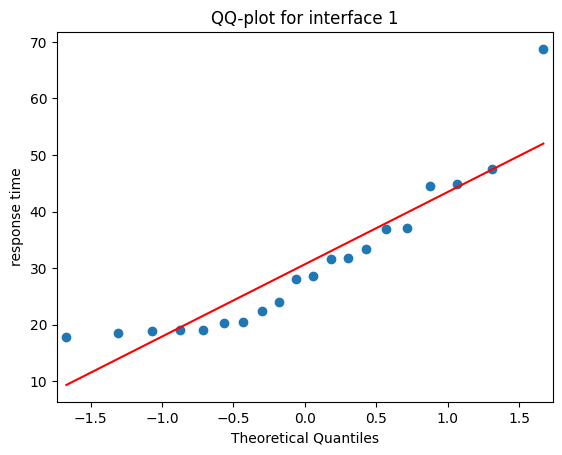
\includegraphics[width=0.9\linewidth, height=6cm]{images/q1QQinterface1.png} 
\caption{QQ-plot for interface1}
\label{fig:q1QQ1}
\end{subfigure}
\begin{subfigure}{0.5\textwidth}
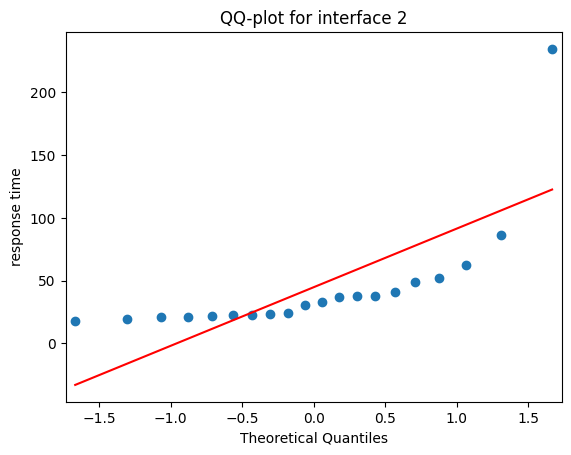
\includegraphics[width=0.9\linewidth, height=6cm]{images/q1QQinterface2.png}
\caption{QQ-plot for interface2}
\label{fig:q1QQ2}
\end{subfigure}
    \caption{QQ-plots for interface1 and interface2}
    \label{fig:enter-label}
\end{figure}
As we can see in figure \ref{fig:q1QQ1}, the data follows the normal distribution for the most part. We see that most response times fall under the normal distribution, but as they are not far apart, I will assume that the data for the first interface follows the normal distribution.
We do have one outlier, the last datapoint (as also shown in the boxplot). As it's only one, we can ignore it for now.
Let us take a look at the QQ plot of the second interface in figure \ref{fig:q1QQ2}. As we can see from the data, it might not be normally distributed. It seems to have a mix of being uniformly distributed (especially at the start) and normally distributed going towards the second half of the range. For the dataset of the second interface, I will assume that it is not normally distributed.
\subsection{Test whether one of the web forms has faster responses. Explain what you did, why, and what the underlying experimental design was. (2+2+2 pts.)}
To test whether one of the web forms has a faster response, we will have to perform a statistical test to compare two samples. Such a test is the two-sample t-test, since we are testing two independent datasets. Let us begin by formulating our hypothesis. \newline\newline
Null hypotheses $H_0$: There is no difference in response times between the two interfaces. \newline
Alternative hypothesis $H_A$: There is a difference in response times between the two interfaces.
We choose $\alpha = 0.05$ as our significance level. \newline\newline
Since the two-sample t-test works under the assumption that both datasets follow the normal distribution, we first have to be able to not reject this assumption. We will do this by performing a Shapiro-Wilk test on both datasets. Let us formulate our hypothesis for the Shapiro-Wilk test. \newline\newline
Null hypotheses $H_{SW0}$: The response times follow the normal distribution. \newline
Alternative hypothesis $H_{SWA}$: The response times do not follow the normal distribution. \newline
We choose $\alpha = 0.05$ as our significance level.\newline\newline
\begin{listing}[H]
\begin{minted}[
baselinestretch=1.2,
frame=lines,
framesep=2mm,
bgcolor=LightGray,
fontsize=\footnotesize,
linenos
]
{python}
from scipy.stats import shapiro
shapiro_1 = shapiro(df['interface1'])
shapiro_2 = shapiro(df['interface2'])
print(f'Shapiro-Wilk test for interface 1: statistic = 
    {shapiro_1.statistic}, p-value = {shapiro_1.pvalue}')
print(f'Shapiro-Wilk test for interface 2: statisitc = 
    {shapiro_2.statistic}, p-value = {shapiro_2.pvalue}')
\end{minted}
\caption{Shapiro-Wilk test}
\label{listing:q1bshapiro}
\end{listing}
The test statistic is $0.855$ for the first interface.
Surprisingly, the data for the first interface does not follow the normal distribution. This is because $p$-$value = 0.007$ and $p$-$value < \alpha$. So we reject our null hypothesis for the first interface. This does, however, contradict our conclusion from the QQ-plot.
Now for the second interface, the test statistic is $0.525$, and the data does not follow the normal distribution either. This is because $p$-$value = 5.46 * 10^{-7}$ and $p$-$value < \alpha$. So we also reject the null hypothesis for the second interface. Consequently, we cannot use the two-sample t-test because our assumption that both datasets follow the normal distribution does not hold. Alternatively, we can use the Mann-Whitney U test, also known as the Wilcoxon rank-sum test, which works under the assumption that at least one of the datasets does not follow the normal distribution.
\begin{listing}[H]
\begin{minted}[
baselinestretch=1.2,
frame=lines,
framesep=2mm,
bgcolor=LightGray,
fontsize=\footnotesize,
linenos
]
{python}
from scipy.stats import mannwhitneyu
mannwhit = mannwhitneyu(df['interface1'], df['interface2'])
print(f'Mann-Whitney U test: statistic = {mannwhit.statistic}, p-value = {mannwhit.pvalue}')
\end{minted}
\caption{Mann-Whitney U test}
\label{listing:q1mannwhitneyu}
\end{listing}
The test statistic from the Mann-Whitney U test is $156$ and the $p$-$value = 0.239$. Since the $p$-$value > \alpha$ we cannot reject our null hypothesis, $H_0$. We conclude that there is not enough evidence to reject the null hypothesis at the $5\%$ significance level and thus cannot say if there is a difference in response times between the two interfaces.
\section{Question 2}
\subsection{General information}
\begin{itemize}
    \item The data file contains the results of comparing two deep learning architectures that were applied to tasks of different levels of complexity (between 100 and 300) and whether the learning managed to converge.
    \item The file used for this question was Question2\_4.txt
\end{itemize}
\subsection{Investigate whether one of the two architectures performs better (i.e. converges for more complex tasks). Explain what you did and why. (5pts.)}
Since we have a dataset with two architectures that are categorised in terms of their complexity and whether they did or did not converge, we can use logistic regression on both groups to determine which one performs better. Let us start with reading the dataset and preparing the data to fit the model.
\begin{listing}[H]
\begin{minted}[
baselinestretch=1.2,
frame=lines,
framesep=2mm,
bgcolor=LightGray,
fontsize=\footnotesize,
linenos
]
{python}
import pandas as pd
from statsmodels.api import Logit
df = pd.read_csv('datasets/Question2_4.txt', sep="\t", header=0)
df['Intercept'] = 1
grouped = df.groupby(df['Architecture'])
\end{minted}
\caption{Reading and preparing data}
\label{listing:q2prep}
\end{listing}
Next up, let us get the independent and dependent variables per group to fit the models. But first, let us formulate our hypotheses for both models. \newline\newline
Null hypothesis $H_0$: The coefficient is not statistically significant. \newline
Alternative hypothesis $H_A$: The coefficient is statistically significant. \newline
We choose $\alpha = 0.05$ as our significance level. \newline\newline
Null hypothesis $H_{I0}$: the baseline log-odds of convergence is not statistically significant. \newline
Alternative hypothesis $H_{IA}$: the baseline log-odds of convergence is statistically significant. \newline
We choose $\alpha = 0.05$ as our significance level. \newline\newline
\begin{listing}[H]
\begin{minted}[
baselinestretch=1.2,
frame=lines,
framesep=2mm,
bgcolor=LightGray,
fontsize=\footnotesize,
linenos
]
{python}
arch1_independant = grouped.get_group('architecture 1')[['Intercept', 'Complexity']]
arch1_dependant = grouped.get_group('architecture 1')['Convergence']
arch2_independant = grouped.get_group('architecture 2')[['Intercept', 'Complexity']]
arch2_dependant = grouped.get_group('architecture 2')['Convergence']
arch_1_model = Logit(arch1_dependant, arch1_independant).fit()
arch_2_model = Logit(arch2_dependant, arch2_independant).fit()
print(arch_1_model.summary())
print(arch_2_model.summary())
\end{minted}
\caption{Fitting the models}
\label{listing:q2Fitmodels}
\end{listing}
\begin{table}[H]
    \centering
\begin{tabular}{ |c|c|c|c|c| }
\hline
\rowcolor{lightgray} \multicolumn{1}{|c|}{} & \multicolumn{2}{|c|}{Architecture 1} &
\multicolumn{2}{|c|}{Architecture 2}\\
\hline
& Intercept & Complexity & Intercept & Complexity \\
\hline
coeff & $-4.1482$ & $0.0164$ & $-3.7368$ & $0.0167$\\
\hline
p-value & 0 & 0 & 0 & 0\\ 
\hline
\end{tabular}
    \caption{Results from the model summary()'s}
    \label{tab:q2results}
\end{table}
As we can see in table \ref{tab:q2results}, the p-values are all 0s and thus smaller than our significance levels. This means that all the null hypotheses from the models are rejected. Consequently, this suggests that the coefficients and the baseline of log-odds are statistically significant. Now, looking at our coefficients, we can conclude that Architecture 2 seems to be just slightly better.
\subsection{At which level of complexity does each architecture converges in 50\% of cases? Explain how you calculated this. (5 pts.)}
\begin{listing}[H]
\begin{minted}[
baselinestretch=1.2,
frame=lines,
framesep=2mm,
bgcolor=LightGray,
fontsize=\footnotesize,
linenos
]
{python}
from math import ceil
complexity_arch_1 = ceil(-arch_1_model.params['Intercept'] / arch_1_model.params['Complexity'])
complexity_arch_2 = ceil(-arch_2_model.params['Intercept'] / arch_2_model.params['Complexity'])
\end{minted}
\caption{Computing complexity level}
\label{listing:q2complexitylevels}
\end{listing}
\begin{itemize}
\centering
    \item The complexity level for architecture 1 to converge in 50\% of cases is 253
    \item The complexity level for architecture 2 to converge in 50\% of cases is 224
\end{itemize}
We know the model's equation, which is $logit = \beta_0 + \beta_1 * Complexity$, where $\beta_0$ is the intercept term, $\beta_1$ is the coefficient for the complexity variable, and $Complexity$ is the predictor variable. Since the inverse logit function is $p = \frac{1}{1 + e^{-logit(p)}}$ and we need to solve for $p = 0.5$, we will get $0.5 = \frac{1}{1 + e^{-logit(p)}}$. Consequently, we can set $logit(p) = 0$ and solve for the predictor variable. To solve $\beta_0 + \beta_1 * Complexity = 0$, we can algebraically transform it to $Complexity = -\frac{\beta_{0}}{\beta_{1}}$ and input the coefficients, which leads to the python code in listing \ref{listing:q2complexitylevels}\footnote{Rounded up due to integers and not fractions}. To verify our solutions, we can also input our complexity levels back into the inverse logit function. $\frac{1}{1 + e^{-(253 * 0.0164 - 4.1482)}} = 0.5$. Analogically, we can also do this for the second architecture, which results in $\frac{1}{1 + e^{-(224 * 0.0167 - 3.7368)}} = 0.5$
\section{Question 3}
\subsection{General information}
\begin{itemize}
\item The data file contains the results of an experiment in which people's acceptance of robots of different degrees of realism is measured.
    \item The dataset used in this question was Question3\_3.txt.
\end{itemize}
\subsection{Make an appropriate plot of the data and explain why this is appropriate (2 pts.)}
To start analysing our data, let us import it first and get some general information to get started.
\begin{listing}[H]
\begin{minted}[
baselinestretch=1.2,
frame=lines,
framesep=2mm,
bgcolor=LightGray,
fontsize=\footnotesize,
linenos
]
{python}
import pandas as pd
df = pd.read_csv('datasets/Question3_3.txt', sep="\t", header=0)
df.describe()
\end{minted}
\caption{Describing the datasets}
\label{listing:q3description}
\end{listing}
\begin{table}[H]
    \centering
    \begin{tabular}{|c|c|c|}
    \hline
    & realism & acceptability \\
    \hline
count & 	$100$	 & $100$\\
\hline
mean & 	$52.17$	 & $68.62$\\
\hline
std	 & $27.99$	 & $28.91$\\
\hline
min	& $1$	& $5$\\
\hline
$25\%$	& $31.75$	& $49.75$\\
\hline
$50\%$	& $52$	& $74$\\
\hline
$75\%$	& $78.25$	& $95$\\
\hline
max	& $98$	& $100$\\
\hline
    \end{tabular}
    \caption{Description of the data}
    \label{tab:q3describe}
\end{table}
For this question, we will not discuss the description as it is not part of the question, but it is still good to have an overview. \newline
For the plot, I chose a scatterplot because it very clearly shows a correlation between the independent variable, the degree of realism, and the dependent variable, acceptability. It also shows the values as a function of an input variable: $f(x)=y$, given that $x\in$ degree of realism and $y\in$ acceptability.
\begin{listing}[H]
\begin{minted}[
baselinestretch=1.2,
frame=lines,
framesep=2mm,
bgcolor=LightGray,
fontsize=\footnotesize,
linenos
]
{python}
import matplotlib.pyplot as plt
plt.scatter(x=df['realism'], y=df['acceptability'])
plt.title('Acceptance of robots in function of its realism')
plt.xlabel('Realism degree')
plt.ylabel('Acceptability')
plt.show()
\end{minted}
\caption{Plotting the scatterplot}
\label{listing:q3scatter}
\end{listing}
\begin{figure}[H]
    \centering
    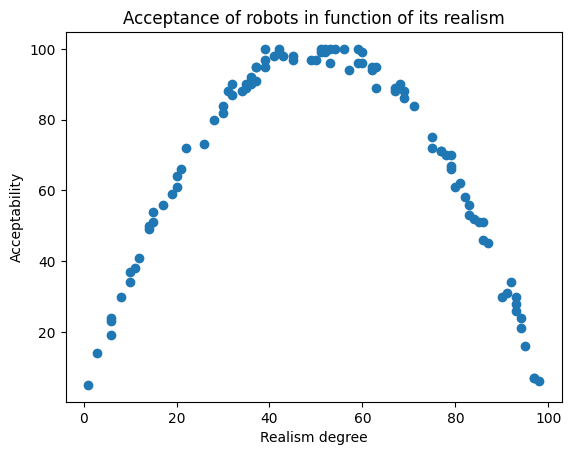
\includegraphics[width=0.8\textwidth]{images/q3scatter.png}
    \caption{Scatterplot showing the acceptance of robots given it's degree of realism}
    \label{fig:q3scatter}
\end{figure}
The correlation we can see is that acceptability is low on the edges of the range, but as it nears the centre, it increases. In some cases, the acceptability is even 100. Kind of like an upside-down quadratic function.
\subsection{Test for correlation between the independent and dependent variables. Pay attention to significance and effect size. Explain what you did and why. (3pts.)}
Since realism is the independent variable and acceptability is the dependent variable, we can use Pearson's correlation coefficient to compute the correlation. However, since the scatterplot showed us an upside-down U-shape, we might not want to use Pearson's correlation coefficient because it assumes a linear relationship, which is not the case. Instead, we can use Spearman's rank correlation coefficient or Kendall's tau. In this case, I chose Spearman's rank correlation coefficient over Kendall's tau because it is more sensitive to repeating pairs. Which we have plenty of, as shown in figure \ref{fig:q3scatter}. First, let us formulate our hypothesis. \newline\newline
Null hypothesis $H_0$: There is no correlation between the independent and dependent variables.  \newline
Alternative hypothesis $H_A$: There is a correlation between the independent and dependent variables. \newline
We choose $\alpha = 0.05$ as our significance level. \newline\newline
\begin{listing}[H]
\begin{minted}[
baselinestretch=1.2,
frame=lines,
framesep=2mm,
bgcolor=LightGray,
fontsize=\footnotesize,
linenos
]
{python}
from scipy.stats import spearmanr
r = spearmanr(df['realism'], df['acceptability'])
print(f"Spearman's Rank Correlation Coefficient: statistic: {r.statistic}, p-value: {r.pvalue}")
\end{minted}
\caption{Spearman's Rank Correlation Coefficient}
\label{listing:q3Spearman}
\end{listing}
The result of the test gives us: S-statistic $= -0.12$ and p-value $= 0.23$. Since the p-value $> \alpha$, we cannot reject our null hypothesis. The S-statistic indicates a nearly negligible negative relationship. We can compute the effect size by using the absolute value of the S-statistic. $|-0.12| = 0.12$. This is a small effect and this suggests that there is a relatively weak relationship between the variables.
\subsection{Discuss whether the outcome of the test corresponds to what you would expect given the data set and the fact that correlation really means that knowing the independent variable tells you something about the dependent variable. What went wrong? (2 pts.)}
The result of the test gives us: S-statistic $= -0.12$ and p-value $= 0.23$. Since the p-value $> \alpha$, we cannot reject our null hypothesis. The S-statistic indicates a nearly negligible negative relationship. We can compute the effect size by using the absolute value of the S-statistic. $|-0.12| = 0.12$. This is a small effect, and this suggests that there is a relatively weak relationship between the variables. However, we can clearly see a strong relationship in the scatterplot.
Alternatively, we could do a Kendall's tau test since it is less affected by tied values; however, I think Spearman's test is more appropriate due to the larger sample size. Regardless, it should have similar results if we use the same hypothesis as before.
\begin{listing}[H]
\begin{minted}[
baselinestretch=1.2,
frame=lines,
framesep=2mm,
bgcolor=LightGray,
fontsize=\footnotesize,
linenos
]
{python}
from scipy.stats import kendalltau
kendalls = kendalltau(df["realism"], df["acceptability"])
print(f"Kendall Tau's: statistic: {kendalls.statistic}, p-value: {kendalls.pvalue}")
\end{minted}
\caption{Kendall Tau's}
\label{listing:q3Kendall}
\end{listing}
With a T-statistic $= -0.08$ and a p-value $= 0.20$. As expected, the test leads to similar results as with Spearman's test. We are still unable to reject the null hypothesis.
\subsection{Explain how you could do a statistical test that works on this kind of data – it is a fairly simple modification of a test you know (3 pts.)}
What we could try is fitting the data to a quadratic function of the form $y= ax^2 + bx + c$, where x is the independent variable (degree of realism) and y is the dependent variable (acceptability), and the rest are coefficients. We can then analyse the goodness of fit, use $R^2$ (coefficient of determination), and perform a statistical test on the coefficients to conclude if there is in fact a correlation. This is called a polynomial regression analysis of degree 2, which might relate to the simpler version, the linear regression analysis.
\section{Question 4}
\subsection{Determine how many samples you need for a t-test on data with an effect size (Cohen's d) of 0.5 to achieve a power of 0.8 with significance 0.05. (2 pts.)}
We can compute this by doing a power analysis on the t-test. In Python, we can use the \newline TtestIndPower class to perform such an analysis, fill in what we know, and it will return the parameter that we do not know.
\begin{listing}[H]
\begin{minted}[
baselinestretch=1.2,
frame=lines,
framesep=2mm,
bgcolor=LightGray,
fontsize=\footnotesize,
linenos
]
{python}
from statsmodels.stats.power import TTestIndPower
from math import ceil
power_analysis = TTestIndPower()
sample_size = ceil(power_analysis.solve_power(effect_size=0.5, power=0.8, alpha=0.05))
print(f'Sample Size: {sample_size}')
\end{minted}
\caption{Computing sample size}
\label{listing:q4power}
\end{listing}
Since the power analysis returns a sample size, which is not an integer but rather a fraction, I will be rounding it up. This is because it does not make sense to have a fraction of a sample size.
The required sample size is 64.
\subsection{Generate 1000 times 2 uniformly distributed samples of this size (assume 100 if you do not know how to calculate the previous answer) with identical means and standard deviations and check how many times a significant difference is found. What is your conclusion about the type I error rate of applying a t-test to uniformly distributed data? (3 pts)}
For this, we will first define the constants that we need for the experiments.
\begin{listing}[H]
\begin{minted}[
baselinestretch=1.2,
frame=lines,
framesep=2mm,
bgcolor=LightGray,
fontsize=\footnotesize,
linenos
]
{python}
import numpy as np
from scipy.stats import ttest_ind

rng = np.random.default_rng(42)
sig = 0.05
reject_count = 0
experiment_count = 0
\end{minted}
\caption{Required constants}
\label{listing:q4consts}
\end{listing}
The random generator has a seed of 42 to be able to repeat the experiment with identical samples. Let's define some functions to aid us in the experiment.
\begin{listing}[H]
\begin{minted}[
baselinestretch=1.2,
frame=lines,
framesep=2mm,
bgcolor=LightGray,
fontsize=\footnotesize,
linenos
]
{python}
def generate_other_sample(sample):
    new_sample = rng.uniform(size=sample_size)
    new_sample = new_sample - new_sample.mean()
    new_sample = sample.mean() + (sample.std() / new_sample.std()) * new_sample
    new_sample = new_sample + (sample.mean() - new_sample.mean())
    return new_sample

def generate_samples(sample_size):
    sample1 = rng.uniform(0, 1, sample_size)
    sample2 = generate_other_sample(sample1)
    return sample1, sample2

def perform_ttest(sample_size, sig):
    s1, s2 = generate_samples(sample_size)
    _, p = ttest_ind(s1, s2)
    return p < sig
\end{minted}
\label{listing:q4funcs}
\caption{Functions to help us}
\end{listing}
The $generate\_other\_sample$\footnote{Inspired from \url{https://stackoverflow.com/questions/51515423/generate-sample-data-with-an-exact-mean-and-standard-deviation}} function takes in a sample and generates another sample that has an equal mean and standard deviation by centering the new sample around it's mean. Then scale it so it has the same standard deviation as the given sample. Finally, we adjust the mean to be the same as the first sample. The $generate\_samples$ just returns two samples with identical means and standard deviation; the perfrom\_ttest function calls the $generate\_samples$ function and performs an independent t-test on the samples. Returning whether the p-value is lower than the significance level. Now for our hypothesis: \newline\newline
Null hypothesis $H_0$: The means are the same.\newline
Alternative hypothesis $H_A$ The means are not equal.\newline
The chosen significance level is 5\%. \newline\newline
When we compute the 1000 experiments, we will add one to our experiment counter and one to our reject counter whenever the test has a p-value lower than the chosen significance level. I expect that since the means are the same and the standard deviation is the same in each pair of samples, the reject counter will never increase.
\begin{listing}[H]
\begin{minted}[
baselinestretch=1.2,
frame=lines,
framesep=2mm,
bgcolor=LightGray,
fontsize=\footnotesize,
linenos
]
{python}
def perform_experiment(sample_size, sig, test):
    global experiment_count
    experiment_count += 1
    if test(sample_size, sig):
        global reject_count
        reject_count += 1
        
for _ in range(1000):
    perform_experiment(sample_size, sig, perform_ttest)
print(f'Experiment count: {experiment_count}')
print(f'Reject count: {reject_count}')
\end{minted}
\label{listing:q4.3.1000exps}
\caption{1000 experiments}
\end{listing}
As expected, after the 1000 experiments, the experiment counter reached 1000, but the reject counter stayed at 0.
\subsection{Generate 1000 times 2 uniformly distributed samples of the above size that are so far apart that the effect size would be 0.5 and count the number of times you find a significant difference. What is your conclusion about the power of applying the t-test to uniformly distributed data? (2 pts)}
Given as background: the variance of the uniform distribution
between a and b is $1/12(b – a)^2$.\newline\newline
For this experiment, we need to generate two samples and introduce the effect size in one of the samples. After that, we perform a two-sample independent t-test like before and sum the number of cases where the p-value is below the significance level. We will use the same hypothesis as before: \newline\newline
Null hypothesis $H_0$: The means are the same.\newline
Alternative hypothesis $H_A$ The means are not equal.\newline
The chosen significance level is $5\%$\newline\newline
\begin{listing}[H]
\begin{minted}[
baselinestretch=1.2,
frame=lines,
framesep=2mm,
bgcolor=LightGray,
fontsize=\footnotesize,
linenos
]
{python}
effect_size = 0.5
experiment_count = 0
reject_count = 0

def perform_ttest_with_effect_size(sample_size, sig):
    s1 = rng.uniform(0,1,sample_size)
    s2 = rng.uniform(0,1,sample_size)
    s2 += effect_size
    _, p = ttest_ind(s1, s2)
    return p < sig

for _ in range(1000):
    perform_experiment(sample_size, sig, perform_ttest_with_effect_size)
print(f'Experiment count: {experiment_count}')
print(f'Reject count: {reject_count}')
print(f'Power: {reject_count / experiment_count}')
\end{minted}
\label{listing:q4.4.1000exps}
\caption{1000 experiments}
\end{listing}
Unsurprisingly, the experiment count and reject count are both 1000.
This is because introducing the effect size to the sample always moves the mean far enough away that the t-test rejects the null hypothesis. Since the experiment count and reject count are the same, the power will be 1.
\subsection{Repeat subquestions 2 and 3 with the Cauchy distribution. As a difference between the two you can use 1. Also repeat subquestion 3 using the Wilcoxon rank sum test. What can you conclude about applying the t-test to Cauchy-distributed data? (3 pts.)}
Given as background: If X is distributed uniformly between 0 and 1, then  $ \tan(\pi (X – \frac{1}{2}))$ follows the Cauchy distribution.\newline\newline
\subsubsection{Cauchy distribution subquestion 2}
Before we can perform this experiment, we define some new functions to generate cauchy samples\footnote{Inspired from \url{https://stackoverflow.com/questions/51515423/generate-sample-data-with-an-exact-mean-and-standard-deviation}} and perform the t-test on these samples.
\begin{listing}[H]
\begin{minted}[
baselinestretch=1.2,
frame=lines,
framesep=2mm,
bgcolor=LightGray,
fontsize=\footnotesize,
linenos
]
{python}
def generate_cauchy_samples(sample_size):
    cauchy1 = rng.standard_cauchy(size=sample_size)
    cauchy2 = rng.standard_cauchy(size=sample_size)
    cauchy2 = cauchy2 - cauchy2.mean()
    cauchy2 = cauchy1.mean() + (cauchy1.std() / cauchy2.std()) * cauchy2
    cauchy2 = cauchy2 + (cauchy1.mean() - cauchy2.mean())
    return cauchy1, cauchy2

def cauchy_ttest(sample_size, sig):
    c1, c2 = generate_cauchy_samples(sample_size)
    _, p = ttest_ind(c1, c2)
    return p < sig
\end{minted}
\label{listing:q4.4.cauchyfuncs}
\caption{Cauchy distributions with identical means and std}
\end{listing}
Next, we perform the 1000 experiments. For these last parts of the experiments, I made use of the multiprocessing library to perform the tests in parallel. Since I experimented with bigger sample sizes, it required more computing power, so it made sense to optimise the experiments more. Be aware that I used Threadpool instead of Pool because I used Jupyter notebook, and Pool does not work in Jupyter notebook. However, I did rename it Pool after the import. Our hypothesis will be: \newline\newline
Null hypothesis $H_0$: The means are the same.\newline
Alternative hypothesis $H_A$ The means are not equal.\newline
The chosen significance level is $5\%$.\newline\newline
\begin{listing}[H]
\begin{minted}[
baselinestretch=1.2,
frame=lines,
framesep=2mm,
bgcolor=LightGray,
fontsize=\footnotesize,
linenos
]
{python}
from multiprocessing.pool import ThreadPool as Pool
experiment_count = 0
reject_count = 
sig = 0.05

pool = Pool()
for _ in range(1000):
    pool.apply_async(perform_experiment, args=(sample_size, sig, cauchy_ttest))
pool.close()
pool.join()

print(f'Experiment count: {experiment_count}')
print(f'Reject count: {reject_count}')
print(f'Type 1 error rate: {reject_count / experiment_count}')
\end{minted}
\label{listing:q4.4.cauchyexps}
\caption{Performing the experiments for the cauchy dists with equal means and std}
\end{listing}
We notice that the number of null hypotheses that are rejected is 0. Therefore, the type 1 error will also be 0. Logically, if we compare the means of two samples where the means are identical and the standard deviations are also the same, then the t-test should have a p-value above 0.05.
\subsubsection{Cauchy distribution subquestion 3}
For these experiments, we will be using an effect size of 0.5. We create a new function that generates two cauchy samples, adds the effect size to the second sample, and then performs a t-test on the samples. The function will then return if the p-value is lower than the significance level.
\begin{listing}[H]
\begin{minted}[
baselinestretch=1.2,
frame=lines,
framesep=2mm,
bgcolor=LightGray,
fontsize=\footnotesize,
linenos
]
{python}
def cauchy_ttest_effect_size(sample_size, sig):
    c1, c2 = rng.standard_cauchy(size=sample_size), rng.standard_cauchy(size=sample_size)
    c2 += effect_size
    _, p = ttest_ind(c1, c2)
    return p < sig
\end{minted}
\label{listing:q4.4.2cauchyfuncs}
\caption{Function to perform a t-test on two cauchy samples, one with effect size}
\end{listing}
Our hypotheses will be: \newline\newline
Null hypothesis $H_0$: The means are the same.\newline
Alternative hypothesis $H_A$ The means are not equal.\newline
The chosen significance level is $5\%$.\newline\newline
\begin{listing}[H]
\begin{minted}[
baselinestretch=1.2,
frame=lines,
framesep=2mm,
bgcolor=LightGray,
fontsize=\footnotesize,
linenos
]
{python}
reject_count = 0
experiment_count = 0
effect_size = 0.5

pool = Pool()
for _ in range(1000):
    pool.apply_async(perform_experiment, args=(sample_size, sig, cauchy_ttest_effect_size))
pool.close()
pool.join()

print(f'Experiment count: {experiment_count}')
print(f'Reject count: {reject_count}')
print(f'Power: {reject_count / experiment_count}')
\end{minted}
\label{listing:q4.4.2cauchyexps}
\caption{Function to perform a t-test on two cauchy samples, one with effect size}
\end{listing}
Contrary to how the t-test performed for the uniform samples, it did not reject all null hypotheses in the experiments but only 34 out of 1000. The power is 0.034. Let us try this again, but with a Wilcoxon rank sum test. Our hypotheses will be: \newline\newline
Null hypothesis $H_0$: The distributions of the two samples are equal.\newline
Alternative hypothesis $H_A$: The distributions of the two samples are not equal.\newline
The chosen significance level is $5\%$.
\begin{listing}[H]
\begin{minted}[
baselinestretch=1.2,
frame=lines,
framesep=2mm,
bgcolor=LightGray,
fontsize=\footnotesize,
linenos
]
{python}
from scipy.stats import mannwhitneyu

experiment_count = 0
reject_count = 0

def cauchy_mannwhitneyu(sample_size, sig):
    c1, c2 = rng.standard_cauchy(size=sample_size), rng.standard_cauchy(size=sample_size)
    c2 += effect_size
    _, p = mannwhitneyu(c1, c2)
    return p < sig
    
pool = Pool()
for _ in range(1000):
    pool.apply_async(perform_experiment, args=(sample_size, sig, cauchy_mannwhitneyu))
pool.close()
pool.join()

print(f'Experiment count: {experiment_count}')
print(f'Reject count: {reject_count}')
print(f'Power: {reject_count / experiment_count}')
\end{minted}
\label{listing:q4.4.2cauchyexpsmannwhit}
\caption{Experiments with cauchy, effect size and wilcoxon}
\end{listing}
After performing these experiments, I found that the null hypothesis has been rejected a total of 317 times, giving it a power of 0.317. We can see that the Wilcoxon rank sum test performs better than the t-test at detecting the effect size. This is most likely due to the fact that the t-test uses the central limit theorem on large samples. The central limit theorem assumes a finite mean and standard deviation, which is not the case with cauchy distributed data, making it unreliable. However, the Wilcoxon rank sum test does not assume a distribution, which makes it more robust to cauchy distributed data.
\section{Appendix A}
\begin{listing}[H]
\begin{minted}[
baselinestretch=1.2,
frame=lines,
framesep=2mm,
bgcolor=LightGray,
fontsize=\footnotesize,
linenos
]
{text}
anyio==4.1.0
argon2-cffi==23.1.0
argon2-cffi-bindings==21.2.0
arrow==1.3.0
asttokens==2.4.1
async-lru==2.0.4
attrs==23.1.0
Babel==2.13.1
beautifulsoup4==4.12.2
bleach==6.1.0
certifi==2023.11.17
cffi==1.16.0
charset-normalizer==3.3.2
colorama==0.4.6
comm==0.2.0
contourpy==1.2.0
cycler==0.12.1
debugpy==1.8.0
decorator==5.1.1
defusedxml==0.7.1
executing==2.0.1
fastjsonschema==2.19.0
fonttools==4.45.1
fqdn==1.5.1
idna==3.6
ipykernel==6.27.1
ipython==8.18.1
isoduration==20.11.0
jedi==0.19.1
Jinja2==3.1.2
json5==0.9.14
jsonpointer==2.4
jsonschema==4.20.0
jsonschema-specifications==2023.11.2
jupyter-events==0.9.0
jupyter-lsp==2.2.1
jupyter_client==8.6.0
jupyter_core==5.5.0
jupyter_server==2.11.1
jupyter_server_terminals==0.4.4
jupyterlab==4.0.9
jupyterlab_pygments==0.3.0
jupyterlab_server==2.25.2
\end{minted}
\end{listing}
\begin{listing}[H]
\begin{minted}[
baselinestretch=1.2,
frame=lines,
framesep=2mm,
bgcolor=LightGray,
fontsize=\footnotesize,
linenos
]
{text}
kiwisolver==1.4.5
MarkupSafe==2.1.3
matplotlib==3.8.2
matplotlib-inline==0.1.6
mistune==3.0.2
nbclient==0.9.0
nbconvert==7.11.0
nbformat==5.9.2
nest-asyncio==1.5.8
notebook==7.0.6
notebook_shim==0.2.3
numpy==1.26.2
overrides==7.4.0
packaging==23.2
pandas==2.1.3
pandocfilters==1.5.0
parso==0.8.3
patsy==0.5.4
Pillow==10.1.0
platformdirs==4.0.0
prometheus-client==0.19.0
prompt-toolkit==3.0.41
psutil==5.9.6
pure-eval==0.2.2
pycparser==2.21
Pygments==2.17.2
pyparsing==3.1.1
python-dateutil==2.8.2
python-json-logger==2.0.7
pytz==2023.3.post1
pywin32==306
pywinpty==2.0.12
PyYAML==6.0.1
pyzmq==25.1.1
referencing==0.31.1
requests==2.31.0
rfc3339-validator==0.1.4
rfc3986-validator==0.1.1
rpds-py==0.13.2
scipy==1.11.4
seaborn==0.13.0
Send2Trash==1.8.2
setuptools==69.0.2
six==1.16.0
sniffio==1.3.0
soupsieve==2.5
stack-data==0.6.3
\end{minted}
\end{listing}
\begin{listing}[H]
\begin{minted}[
baselinestretch=1.2,
frame=lines,
framesep=2mm,
bgcolor=LightGray,
fontsize=\footnotesize,
linenos
]
{text}
statsmodels==0.14.0
terminado==0.18.0
tinycss2==1.2.1
tornado==6.4
traitlets==5.14.0
types-python-dateutil==2.8.19.14
tzdata==2023.3
uri-template==1.3.0
urllib3==2.1.0
wcwidth==0.2.12
webcolors==1.13
webencodings==0.5.1
websocket-client==1.6.4
\end{minted}
\label{listing:reqs}
\caption{Libraries and dependancies}
\end{listing}
\end{document}